% This must be in the first 5 lines to tell arXiv to use pdfLaTeX, which is strongly recommended.
%\pdfoutput=1
% In particular, the hyperref package requires pdfLaTeX in order to break URLs across lines.

\documentclass[11pt]{article}

% Remove the "review" option to generate the final version.
\usepackage{acl}

% Standard package includes
\usepackage{times}
\usepackage{latexsym}

% For proper rendering and hyphenation of words containing Latin characters (including in bib files)
\usepackage[T1]{fontenc}
% For Vietnamese characters
% \usepackage[T5]{fontenc}
% See https://www.latex-project.org/help/documentation/encguide.pdf for other character sets

% This assumes your files are encoded as UTF8
\usepackage[utf8]{inputenc}

% This is not strictly necessary, and may be commented out,
% but it will improve the layout of the manuscript,
% and will typically save some space.
\usepackage{microtype}

% If the title and author information does not fit in the area allocated, uncomment the following
%
%\setlength\titlebox{<dim>}
%
% and set <dim> to something 5cm or larger.

\usepackage{graphicx}

\title{Discriminating 3D-objects using }

% Author information can be set in various styles:
% For several authors from the same institution:
% \author{Author 1 \and ... \and Author n \\
%         Address line \\ ... \\ Address line}
% if the names do not fit well on one line use
%         Author 1 \\ {\bf Author 2} \\ ... \\ {\bf Author n} \\
% For authors from different institutions:
% \author{Author 1 \\ Address line \\  ... \\ Address line
%         \And  ... \And
%         Author n \\ Address line \\ ... \\ Address line}
% To start a seperate ``row'' of authors use \AND, as in
% \author{Author 1 \\ Address line \\  ... \\ Address line
%         \AND
%         Author 2 \\ Address line \\ ... \\ Address line \And
%         Author 3 \\ Address line \\ ... \\ Address line}

\author{Dominik Künkele \\
  Affiliation / Address line 1 \\
  Affiliation / Address line 2 \\
  Affiliation / Address line 3 \\
  \texttt{dominik.kuenkele@outlook.com} \\\And
  Simon Dobnik \\
  Affiliation / Address line 1 \\
  Affiliation / Address line 2 \\
  Affiliation / Address line 3 \\
  \texttt{simon.dobnik@gu.se} \\}

\begin{document}
\maketitle
\begin{abstract}

\end{abstract}

\section{Introduction}
% TODO:
% \begin{itemize}
%   \item how can models reidentify attributes (and objects) from learned encodings in an artificial language \textbf{(done)}
%   \end{itemize}

Agents interact with the physical world through their action and perception and with other agents through language.
Their sensors and actuators (if they are artificial agents but the same also holds for natural agents) allow them to sample the world and their their own state using measures that are continuous in nature such as intensity of light, distance, angles, velocity and others which can be measured with a high degree of accuracy.
On the other hand language that is used to communicta ewith other agents is based on representations that are composed of a limited set of discrete symbols.
How can both domains and representations arising from these interaction be combined? How are ranges of measurements exprseed in a continuous domain mapped to discrete linguistic labels?
How is ambiguity and underpecification resolved?
Ho can agents achive this through interactive grounding \citep{Regier:1996,Roy:2005,Cooper:2023aa}?

% SD 2023-07-08 14:11:44 +0200: A tip for writing LateX on Git: write each sentence in a separate line, this way any edits and conflicts will be much easier to spot and edit that comparing entire paragraphs.

% \section{Background and previous work}

Language games with a sender and a receiver \citep{Clark:1996aa,Bartlett:2005aa,Kirby:2008ab,SteelsLoetzsch:2009,Zaslavsky:2018aa} offer an opportunity to examine how neural models condense seen information into a distinct representation of symbols through linguistic interaction.
A sender describes a perceptual situation that can also be seen by a receiver starting with a random label while
the receiver attempts to interpret the meaning of these symbols and combine it with other information.
It then sends feedback to the sender about its interpretation.
Interaction is optimised based on the communicative success of the sender and the receiver.
Gradually, both agents converge on a set of symbols that they can use to refer to situations in jointly attended perceptual scenes \citep{Chai:2016aa,Kelleher:2020aa}.
Communication is successful and grounding converges because learning is constrained by joint attention and the agents are playing following the rule of the communicative games.

In this this paper we explore how agents based on artificial neural networks learn referential grounding of entitities in images of 3-dimensional scenes where one agent is discribing the entities and the other agent learns to interpret the reference of symbols in the scene either by identifying the object in the scene as a bounding box or location of the object based on object attributes such as shape, colour and size.
% studies how the agents can encode real-looking objects into distinct symbols and decode this message to reidentify this object. Specifically, the study explores discrimination games using an extended version of the CLEVR dataset, focusing on the identification and differentiation of objects based on their attributes such as shape, color, and size.
The novelty of our work compared with the previous work with this setup \citep{Kharitonov2019} is that (i) we extend the popular CLEVR dataset \citep{Johnson2016} with new artificially generated 3-d scenes of objects that that can be referred to and discriminated based on the attributes such as shape, colour and size whereby the discrimination is based on different overalaps of these attributes between the target and the distractor objects; and (ii) we implement a focused referring to objects aither as one of the potential bounding boxes or location of the target.

% SD 2023-07-08 15:05:37 +0200: This hasn't been studied and implemented by lazaridou and others in the EGG framework, right?

% SD 2023-07-08 15:15:46 +0200: Just saw that we are only reporting on object from bounding box identification and not location, right?

% \section{Materials and methods}
% TODO:
% \begin{itemize}
%   \item creation of dataset (CLEVR) \textbf{(done)}
%         \begin{itemize}
%           \item multiple 'real' objects in scene \textbf{(done)}
%           \item 3 attributes (color, size, shape) differentiate objects \textbf{(done)}
%           \item using 'dale' setup to uniquely identify target object \textbf{(done)}
%           \item extracting bounding boxes \textbf{(done)}
%         \end{itemize}
%   \item building a language game using EGG \textbf{(done)}
%   \item based on feature extractors ResNet \textbf{(done)}
%   \item setup of discriminating game of objects in image \textbf{(done)}
%   \item message encoder/decoder is auto-encoder
% \end{itemize}

\section{Our dataset: CLEVR-DaleTwo and DaleFive}

% SD 2023-07-08 14:58:04 +0200: Rephrase this paragraph to continue from the previous section and emphasise our extension and contribution to the dataset. For our experiments we extend...

The dataset used for these experiments is an extended version of the CLEVR dataset \citep{Johnson2016}.\footnote{%The extended source code can be found on GitHub:
  \href{https://github.com/DominikKuenkele/MLT\_Master-Thesis\_clevr-dataset-gen}{https://github.com/DominikKuenkele/MLT\_Master-Thesis\_clevr-dataset-gen}}
This dataset includes 3D-generated images depicting scenes with different kinds of objects. Each of these objects has different combinations of attributes, such as \emph{shape}, \emph{color} and \emph{size}. The objects are randomly placed into the scene and assigned with random attributes.
Figure \ref{fig:clevr-extended_example} shows an example of a generated image of this CLEVR dataset. The dataset also contains ground truth information about each image, including attributes and locations for all objects.

\begin{figure}[h]
  \centering
  \frame{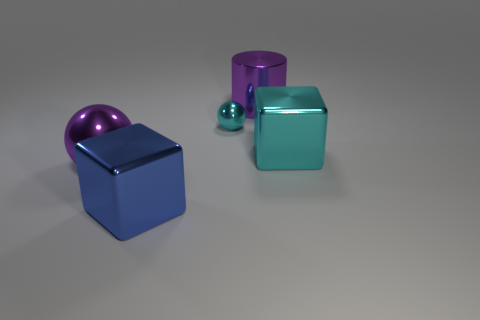
\includegraphics[width=.8\linewidth]{figures/CLEVR_extended_example.png}}
  \caption{Example of a generated image with the extended code} % SD 2023-07-08 15:00:20 +0200: What dataset: Dale-2?
  \label{fig:clevr-extended_example}
\end{figure}

The extended version of the dataset divides the objects into \emph{target object} and \emph{distractors}. The target object is the main object in the scene that should be identified and communicated by the agents. The distractors contain similar objects to the target object. The number of shared attributes is defined by rules researched in \citet{Dale1995}. The target object is therefore always identifiable using either only the \emph{shape} (1), the \emph{shape} and \emph{color} (2) or the \emph{shape}, \emph{color} and \emph{size} (3).

For this research, two datasets are created. The \emph{DaleTwo} dataset contains one target object and one distractor, while the \emph{DaleFive} dataset contains one target object and four distractors. Both datasets contain 10.000 images. For each image fixed size bounding boxes around each object are extracted. These bounding boxes are the input for the sender and receiver in the language game.

% SD 2023-07-08 15:23:38 +0200: Describe a bit more how DaleTwo and DaleFive differ, in particular how many attributes are shared and how between the objects in the DaleFive?

\subsection{Language game}
The language game was developed and run in the EGG framework \citep{Kharitonov2019}. The setup of the game is based on the game described in the paper by \citet{Lazaridou2016}. The same multiple images are passed to a sender and a receiver. The sender must communicate the target image to the receiver with a message, who needs to identify this target image. Instead of distinguishing two images from different concepts, in this experiment the agents need to distinguish two objects with shared attributes. Both sender and receiver have a similar architecture to the \emph{agnostic sender} and \emph{receiver} in \citet{Lazaridou2016}. One central difference is the production of the message. Their paper focuses on the classification of a concept for the input image and therefore produces only one-symbol messages that should correspond to these concepts. This research focuses on the identification of attributes for the objects and their combination, which is why our models produce a sequence of symbols for the message (which may correspond to the attributes). This is done using an encoder LSTM (sender) and a decoder LSTM (receiver) (see Figure \ref*{todo}).

% SD 2023-07-08 15:09:29 +0200: We have now already said some of this in the introduction. In the introduction we can describe the general setup of language games and here we say explicitly what is our configuration and emphasise in particular in what ways it is different from the previously implemented games. Including a list of technical details of the models is great. When restructuign sentences, copy those that fit the previous section there (and comment one out if necessary) and keep the rest here. It requires a bit of strategic thinking where to mention things in such a short paper so that we only say it once and save space.

The initial state of the encoder LSTM is the image, passed through ResNet101 and a following linear layer that reduces the dimensions. The sequence is then created through Gumbel-Softmax relaxation \citep{Jang2016}.

The receiver on the other side takes the sequence as input for its decoder LSTM. The hidden state is randomly initialized. After each step of the LSTM, the receiver calculates the dot product between the hidden state and its own image encoding (calculated as the sender's image encoding). The receiver then 'points' to one of the images, while applying the softmax function over the results. The loss is calculated using the NLL-loss. Following, the losses for each token in the message sequence are summed up, and all weights of the receiver as well as the sender are updated, based on this summed loss.

There are five variables in the experiments that are adjusted: (1) the image embedding size for the sender $e_s$, (2) the LSTM hidden size for the sender $h_s$, (3) the image/message embedding size for the receiver $e_r$, (4) the LSTM hidden size for the receiver $h_r$ and (5) the size of the vocabulary $|V|$.

The results will be evaluated using the accuracy if the receiver could identify the target object. A random guess corresponds to 50\% in the \emph{DaleTwo} dataset and 20\% in the \emph{DaleFive} dataset.

\section{Results}
TODO:
\begin{itemize}
  \item DaleTwo: \textbf{(done)}
        \begin{itemize}
          \item small hidden/embedding dims, small vocab -> high accuracy
          \item high hidden/embedding dims, small vocab -> low accuracy
        \end{itemize}
  \item DaleFive: \textbf{(done)}
        \begin{itemize}
          \item small hidden/embedding dims, small vocab -> low accuracy
          \item small hidden/embedding dims, bigger vocab -> higher accuracy
        \end{itemize}
  \item ... test different hidden/embedding dims
  \item ... test 3/4 objects
\end{itemize}

\begin{table}
  \centering
  \begin{tabular}{c|ccccc|c}
    \hline
    \textbf{Dataset} & $h_{s}$ & $e_{s}$ & $h_{r}$ & $e_{r}$ & $|V|$ & \textbf{Acc.} \\
    \hline
    DaleTwo          & {10}    & {10}    & {10}    & {10}    & {10}  & {95\%}        \\
    DaleTwo          & {50}    & {50}    & {128}   & {128}   & {10}  & {50\%}        \\
    DaleFive         & {10}    & {10}    & {10}    & {10}    & {10}  & {23\%}        \\
    DaleFive         & {10}    & {10}    & {10}    & {10}    & {20}  & {23\%}        \\
    DaleFive         & {10}    & {10}    & {10}    & {10}    & {100} & {41\%}        \\
    \hline
  \end{tabular}
  \caption{Result of the experiments with different hidden sizes, embedding sizes and vocabulary sizes}
  \label{tab:results}
\end{table}

The results of the experiments are summarized in Table \ref{tab:results}. For the \emph{DaleTwo} dataset it can be clearly seen that very small embedding and hidden sizes are beneficial for identifying the correct object. The receiver identifies indeed almost every sample correctly with all sizes of 10. When the hidden and embedding sizes are increased, the guesses by the receiver are random. Interestingly, a vocab size of 10 is enough to communicate a meaningful message for the \emph{DaleTwo} dataset.

% SD 2023-07-08 15:17:45 +0200: The hidden size is related to the vocabulary size. Both have to be optimally selected for the models to converge.

The result change, when using the \emph{DateFive} dataset with four distractors. With low hidden, embedding and vocab size, the agents barely pass the random baseline with 23\%. Only increasing the vocabulary size to 100 raises the accuracy by almost 20\% to 43\%. This accuracy is still far lower than the 95\% with the \emph{DaleTwo} dataset.

% SD 2023-07-08 15:18:24 +0200: So we are not using just two objects to discriminate with as stated in the introduction and the previous section.

% SD 2023-07-08 15:19:05 +0200: Why is the accuarcy lower? One of the reason of course is that there is more uncertanty and the networks have to learn how different combinations of labels that will be up to n! relate to individual perceptual features that are encoded in the linguistic categories. Since we discrimnate objects based on properties that are also distinguished in human cognition (colour, size, shape) we expect that the vocabulary onto which the agents will converge will reflect these catgories anf therefore be close to human vocabulary. We will imnvestiaget the overlap between the vocabularies in our ongoing and future work.

\section{Discussion}
TODO:
\begin{itemize}
  \item maybe calculation of loss (multiplicating instead of summing loss per token), unlikely, since sequence length short -> shouldn't result in big differences
  \item reducing dims of image better the increasing dims of message, increasing dims is not learnable for models
  \item Vocab:
        \begin{itemize}
          \item vocabulary could describe attributes of target image (non-discriminative) or describe only differences (discriminative)
          \item in second case, two images is a far easier task than five images. Hence, much lower accuracy
        \end{itemize}
\end{itemize}

Two interesting conclusions can be drawn. First, the hidden as well as the embedding sizes need not be bigger than the vocabulary size. Even though that means that the image encodings of 4096 or even higher dimensions need to be compressed to fit the vocabulary size, this will still help to produce and interpret more meaningful messages. The reason for this is very likely that neural models have difficulties to upscale from lower dimensions (e.g. from low $h_r$ to high $e_r$).

The second conclusion that can be drawn looks at the difference between the two datasets. Unsurprisingly, the agents have a much higher difficulty to discriminate a target object from four instead of one object. Still the difference in the necessary vocabulary size is striking. There are 48 possible objects. Still a vocabulary size of only 10 is enough for an almost perfect accuracy with two objects. This hints to the fact, that the agents don't describe the complete target object, but only rely on discriminating attributes between the objects. This gets more complex when the agents need to discriminate between five objects. A bigger vocabulary offers a bigger space


\section{Conclusions and further work}

\section*{Acknowledgements}

% Entries for the entire Anthology, followed by custom entries
\bibliography{anthology,custom}


\appendix

\section{Example Appendix}


\end{document}
%%% Local Variables: 
%%% coding: utf-8
%%% mode: latex
%%% mode: flyspell
%%% ispell-local-dictionary: "british"
%%% TeX-engine: default
%%% TeX-master: t
%%% TeX-PDF-mode: t
%%% TeX-command-extra-options: "-shell-escape"
%%% End:
